
\documentclass[a4paper,11pt]{article}
\usepackage[a4paper, margin=8em]{geometry}

% usa i pacchetti per la scrittura in italiano
\usepackage[french,italian]{babel}
\usepackage[T1]{fontenc}
\usepackage[utf8]{inputenc}
\frenchspacing 

% usa i pacchetti per la formattazione matematica
\usepackage{amsmath, amssymb, amsthm, amsfonts}

% usa altri pacchetti
\usepackage{gensymb}
\usepackage{hyperref}
\usepackage{standalone}

\usepackage{colortbl}

\usepackage{xstring}
\usepackage{karnaugh-map}

% imposta il titolo
\title{Appunti Calcolatori Elettronici}
\author{Luca Seggiani}
\date{2025}

% imposta lo stile
% usa helvetica
\usepackage[scaled]{helvet}
% usa palatino
\usepackage{palatino}
% usa un font monospazio guardabile
\usepackage{lmodern}

\renewcommand{\rmdefault}{ppl}
\renewcommand{\sfdefault}{phv}
\renewcommand{\ttdefault}{lmtt}

% circuiti
\usepackage{circuitikz}
\usetikzlibrary{babel}

% testo cerchiato
\newcommand*\circled[1]{\tikz[baseline=(char.base)]{
            \node[shape=circle,draw,inner sep=2pt] (char) {#1};}}

% disponi il titolo
\makeatletter
\renewcommand{\maketitle} {
	\begin{center} 
		\begin{minipage}[t]{.8\textwidth}
			\textsf{\huge\bfseries \@title} 
		\end{minipage}%
		\begin{minipage}[t]{.2\textwidth}
			\raggedleft \vspace{-1.65em}
			\textsf{\small \@author} \vfill
			\textsf{\small \@date}
		\end{minipage}
		\par
	\end{center}

	\thispagestyle{empty}
	\pagestyle{fancy}
}
\makeatother

% disponi teoremi
\usepackage{tcolorbox}
\newtcolorbox[auto counter, number within=section]{theorem}[2][]{%
	colback=blue!10, 
	colframe=blue!40!black, 
	sharp corners=northwest,
	fonttitle=\sffamily\bfseries, 
	title=Teorema~\thetcbcounter: #2, 
	#1
}

% disponi definizioni
\newtcolorbox[auto counter, number within=section]{definition}[2][]{%
	colback=red!10,
	colframe=red!40!black,
	sharp corners=northwest,
	fonttitle=\sffamily\bfseries,
	title=Definizione~\thetcbcounter: #2,
	#1
}

% disponi codice
\usepackage{listings}
\usepackage[table]{xcolor}

\definecolor{codegreen}{rgb}{0,0.6,0}
\definecolor{codegray}{rgb}{0.5,0.5,0.5}
\definecolor{codepurple}{rgb}{0.58,0,0.82}
\definecolor{backcolour}{rgb}{0.95,0.95,0.92}

\lstdefinestyle{codestyle}{
		backgroundcolor=\color{black!5}, 
		commentstyle=\color{codegreen},
		keywordstyle=\bfseries\color{magenta},
		numberstyle=\sffamily\tiny\color{black!60},
		stringstyle=\color{green!50!black},
		basicstyle=\ttfamily\footnotesize,
		breakatwhitespace=false,         
		breaklines=true,                 
		captionpos=b,                    
		keepspaces=true,                 
		numbers=left,                    
		numbersep=5pt,                  
		showspaces=false,                
		showstringspaces=false,
		showtabs=false,                  
		tabsize=2
}

\lstdefinestyle{shellstyle}{
		backgroundcolor=\color{black!5}, 
		basicstyle=\ttfamily\footnotesize\color{black}, 
		commentstyle=\color{black}, 
		keywordstyle=\color{black},
		numberstyle=\color{black!5},
		stringstyle=\color{black}, 
		showspaces=false,
		showstringspaces=false, 
		showtabs=false, 
		tabsize=2, 
		numbers=none, 
		breaklines=true
}


\lstdefinelanguage{assembler}{ 
  keywords={AAA, AAD, AAM, AAS, ADC, ADCB, ADCW, ADCL, ADD, ADDB, ADDW, ADDL, AND, ANDB, ANDW, ANDL,
        ARPL, BOUND, BSF, BSFL, BSFW, BSR, BSRL, BSRW, BSWAP, BT, BTC, BTCB, BTCW, BTCL, BTR, 
        BTRB, BTRW, BTRL, BTS, BTSB, BTSW, BTSL, CALL, CBW, CDQ, CLC, CLD, CLI, CLTS, CMC, CMP,
        CMPB, CMPW, CMPL, CMPS, CMPSB, CMPSD, CMPSW, CMPXCHG, CMPXCHGB, CMPXCHGW, CMPXCHGL,
        CMPXCHG8B, CPUID, CWDE, DAA, DAS, DEC, DECB, DECW, DECL, DIV, DIVB, DIVW, DIVL, ENTER,
        HLT, IDIV, IDIVB, IDIVW, IDIVL, IMUL, IMULB, IMULW, IMULL, IN, INB, INW, INL, INC, INCB,
        INCW, INCL, INS, INSB, INSD, INSW, INT, INT3, INTO, INVD, INVLPG, IRET, IRETD, JA, JAE,
        JB, JBE, JC, JCXZ, JE, JECXZ, JG, JGE, JL, JLE, JMP, JNA, JNAE, JNB, JNBE, JNC, JNE, JNG,
        JNGE, JNL, JNLE, JNO, JNP, JNS, JNZ, JO, JP, JPE, JPO, JS, JZ, LAHF, LAR, LCALL, LDS,
        LEA, LEAVE, LES, LFS, LGDT, LGS, LIDT, LMSW, LOCK, LODSB, LODSD, LODSW, LOOP, LOOPE,
        LOOPNE, LSL, LSS, LTR, MOV, MOVB, MOVW, MOVL, MOVSB, MOVSD, MOVSW, MOVSX, MOVSXB,
        MOVSXW, MOVSXL, MOVZX, MOVZXB, MOVZXW, MOVZXL, MUL, MULB, MULW, MULL, NEG, NEGB, NEGW,
        NEGL, NOP, NOT, NOTB, NOTW, NOTL, OR, ORB, ORW, ORL, OUT, OUTB, OUTW, OUTL, OUTSB, OUTSD,
        OUTSW, POP, POPL, POPW, POPB, POPA, POPAD, POPF, POPFD, PUSH, PUSHL, PUSHW, PUSHB, PUSHA, 
				PUSHAD, PUSHF, PUSHFD, RCL, RCLB, RCLW, MOVSL, MOVSB, MOVSW, STOSL, STOSB, STOSW, LODSB, LODSW,
				LODSL, INSB, INSW, INSL, OUTSB, OUTSL, OUTSW
        RCLL, RCR, RCRB, RCRW, RCRL, RDMSR, RDPMC, RDTSC, REP, REPE, REPNE, RET, ROL, ROLB, ROLW,
        ROLL, ROR, RORB, RORW, RORL, SAHF, SAL, SALB, SALW, SALL, SAR, SARB, SARW, SARL, SBB,
        SBBB, SBBW, SBBL, SCASB, SCASD, SCASW, SETA, SETAE, SETB, SETBE, SETC, SETE, SETG, SETGE,
        SETL, SETLE, SETNA, SETNAE, SETNB, SETNBE, SETNC, SETNE, SETNG, SETNGE, SETNL, SETNLE,
        SETNO, SETNP, SETNS, SETNZ, SETO, SETP, SETPE, SETPO, SETS, SETZ, SGDT, SHL, SHLB, SHLW,
        SHLL, SHLD, SHR, SHRB, SHRW, SHRL, SHRD, SIDT, SLDT, SMSW, STC, STD, STI, STOSB, STOSD,
        STOSW, STR, SUB, SUBB, SUBW, SUBL, TEST, TESTB, TESTW, TESTL, VERR, VERW, WAIT, WBINVD,
        XADD, XADDB, XADDW, XADDL, XCHG, XCHGB, XCHGW, XCHGL, XLAT, XLATB, XOR, XORB, XORW, XORL},
  keywordstyle=\color{blue}\bfseries,
  ndkeywordstyle=\color{darkgray}\bfseries,
  identifierstyle=\color{black},
  sensitive=false,
  comment=[l]{\#},
  morecomment=[s]{/*}{*/},
  commentstyle=\color{purple}\ttfamily,
  stringstyle=\color{red}\ttfamily,
  morestring=[b]',
  morestring=[b]"
}

\lstset{language=assembler, style=codestyle}

% disponi sezioni
\usepackage{titlesec}

\titleformat{\section}
	{\sffamily\Large\bfseries} 
	{\thesection}{1em}{} 
\titleformat{\subsection}
	{\sffamily\large\bfseries}   
	{\thesubsection}{1em}{} 
\titleformat{\subsubsection}
	{\sffamily\normalsize\bfseries} 
	{\thesubsubsection}{1em}{}

% tikz
\usepackage{tikz}

% float
\usepackage{float}

% grafici
\usepackage{pgfplots}
\pgfplotsset{width=10cm,compat=1.9}

% disponi alberi
\usepackage{forest}

\forestset{
	rectstyle/.style={
		for tree={rectangle,draw,font=\large\sffamily}
	},
	roundstyle/.style={
		for tree={circle,draw,font=\large}
	}
}

% disponi algoritmi
\usepackage{algorithm}
\usepackage{algorithmic}
\makeatletter
\renewcommand{\ALG@name}{Algoritmo}
\makeatother

% disponi numeri di pagina
\usepackage{fancyhdr}
\fancyhf{} 
\fancyfoot[L]{\sffamily{\thepage}}

\makeatletter
\fancyhead[L]{\raisebox{1ex}[0pt][0pt]{\sffamily{\@title \ \@date}}} 
\fancyhead[R]{\raisebox{1ex}[0pt][0pt]{\sffamily{\@author}}}
\makeatother

\begin{document}
% sezione (data)
\section{Lezione del 17-03-25}

% stili pagina
\thispagestyle{empty}
\pagestyle{fancy}

% testo
\subsection{Protezione}
Tutti i programmi che abbiamo visto finora hanno il pieno controllo su la macchina su cui sono in esecuzione.
Questo significa che possono impattare qualsiasi regione di memoria, incluso il loro stesso codice macchina, o i frame di stack di programmi lanciati prima di loro.

Un approccio di questo tipo non è ideale quando più programmi, magari di utenti diversi, vengono lanciati ed eseguiti \textit{quasi} in contemporanea (\textit{time-sharing}) sulla stessa macchina.

Un esempio di questa situazione può verificarsi nel caso di esecuziono \textit{batch}, cioè di esecuzione successiva di più programmi, magari scritti da più utenti.
Vorremmo massimizzare l'uso della CPU sospendendo un programma e iniziandone un altro nel caso il primo fra questi inizi un'operazione che richiede una quantità significativa di tempo (ad esempio un accesso a un dispositivo di I/O).
In questo caso, visto che non possiamo fidarci della benevolenza degli utenti nell'inserire istruzioni esplicite per il cambio da un programma all'altro, vorremo agire sull'hardware per, ad esempio, vietare all'utente l'uso di certe istruzioni (qui \lstinline|IN| e \lstinline|OUT|) e costringerlo ad usare primitive messe a disposizione dal sistema.

Chiaramente, però, le primitive dovranno poter usare \lstinline|IN| e \lstinline|OUT| per fare l'I/O vero e proprio con i dispositivi.
Per permettere questo doppio comportamento introduciamo l'idea di \textbf{protezione}.

\subsubsection{Contesti di esecuzione}
Il programma nella memoria potrà essere in esecuzione, in un momento qualsiasi, in uno di due \textbf{contesti}, o \textit{modi} (vedremo nell'architettura x86 corrente, si parla di protezione a \textit{ring}): il contesto \textbf{sistema} e il contesto \textbf{utente}.
Le istruzioni di cui permetterà l'esecuzione saranno quindi determinate dal contesto corrente.

Forniamo allora il processore di un apposito registro, il \textbf{CS} (\textit{Code Segment}), a 2 bit.
I 2 bit sono necessari in quanto storicamente (il meccanismo descritto viene introdotto nell'architettura x86 a partire dal 286) si definivano quattro contesti, o \textbf{ring}:
\begin{table}[h!]
	\center \rowcolors{2}{white}{black!10}
	\begin{tabular} { c | c | c }
		\bfseries CS & \bfseries Ring & \bfseries Tipo \\
		\hline 
		00 & Ring 0 & Kernel (sistema) \\
		01 & Ring 1 & Driver \\
		10 & Ring 2 &  / / \\
		11 & Ring 3 & Utente \\
	\end{tabular}
\end{table}

Il nome CS deriva dal fatto che questo registro era pensato per gestire la \textit{segmentazione} della memoria.
Sia questo meccanismo, che i due ring interni (l'1 e il 2) sono pressoché inutilizzati nell'architettura x86-64 moderna, e quindi li ignoreremo, portandoci effettivamente alla situazione dove CS rappresenta un flag che distingue fra contesto \textit{sistema} e contesto \textit{utente}, come avevamo ipotizzato.

\subsubsection{Transizioni fra contesti}
Ipotizziamo quindi che all'avvio si parta in contesto sistema, e che si passi al contesto utente quando si esegue un programma utente, 
Per permettere all'utente di "accedere" alle istruzioni privilegiate, vogliamo che questo disponga di un modo di tornare al contesto sistema, ma lasciando il controllo al sistema operativo (altrimenti sarebbe inutile introdurre l'idea di un contesto utente in primo luogo).
Di contro, vogliamo un modo per il sistema operativo di restituire in sicurezza il controllo al programma, previa transizione del processore in contesto utente.

Vediamo come il meccanismo dell'interruzione fornisce un metodo per gestire questa situazione.

Introdurremo un tipo di interruzione apposito, che restituisce il controllo al sistema operativo (semplicemente passando ad un gestore di interruzione definito dal sistema operativo) passando a contesto sistema.
Il tipo di operazione che stiamo richedendo al sistema operativo potrà essere passato in qualche registro specifico, solitamente \lstinline|%EAX|.
Il problema potrebbe essere chiaramente che l'utente ha la possibilità di modificare tutta la memoria, e quindi la stessa IDT e il gestore impostato.

\subsubsection{Protezione di memoria}
Si rende quindi necessario un meccanismo di gestione degli accessi in memoria.
In contesto utente, quindi, oltre a permettere l'utilizzo di solo alcune istruzioni \textit{non privilegiate}, il processore dovrà permettere l'accesso solo a determinate regioni di memoria. 
Visto che non abbiamo ancora introdotto l'idea di \textit{memoria virtuale}, modellizziamo temporaneamente questa configurazione con un apposito registro a controllo sistema che decide quali regioni di memoria sono o non sono accessibili.

Abbiamo quindi l'immagine completa del meccanismo della protezione, che avevamo introdotto per privilegiare le sole istruzioni, ma ci rendiamo adesso conto deve consistere in:
\begin{itemize}
	\item Protezione delle \textbf{istruzioni} attraverso il loro privilegiamento al contesto sistema, come avevamo visto;
	\item Protezione della \textbf{memoria} definendo regioni accessibili in sola modalità sistema.
\end{itemize}

\subsubsection{Transizione da contesto utente a contesto sistema}
Vediamo nel dettaglio come si passa dal contesto utente al contesto sistema.
Per questo sfrutteremo l'istruzione x86 \lstinline|INT|, che permette di generare un interruzione software sulla base del tipo fornito come operando.
Si potrà quindi implementare il meccanismo della \textit{chiamata a sistemo}, secondo una modalità del tipo:
\begin{lstlisting}[language=assembler, style=codestyle]	
mov $0x00, %eax # tipo chiamata
int $0x80       # chiamata sistema (per x86, in x86-64 esiste syscall)
\end{lstlisting}
Notiamo che questo è l'approccio normalmente supportato dai moderni sistemi operativi x86 (specialmente Linux, anche se oggi si usa l'istruzione apposita \lstinline|syscall|).
Vedremo che il passaggio del tipo chiamata nel registro \lstinline|%EAX| non si verifica nel kernel che studieremo, dove invece ognuno dei 224 tipi di interruzioni liberi potrà rappresentare una chiamata a sistema diversa.

Questo si tradurrà a livello processore nel salvataggio dello stato corrente di esecuzione, la transizione al contesto sistema e lo spostamento in IP della prima istruzione di un apposito sottoprograma di servizio atto a gestire l'eccezione (e quindi soddisfare, se possibile, la richiesta del programma per cui questo ha sollevato in primo luogo l'interruzione).

Per capire nel dettaglio cosa accade nel processore è necessario:
\begin{itemize}
	\item Capire come è strutturata la Interrupt Descriptor Table (IDT) all'interno della memoria del sistema, che supponiamo essere privilegiata (altrimenti l'utente potrebbe manometterla);
	\item Capire come viene gestita un interruzione software, cioè come si conserva lo stato al momento dell'interruzione, e come si inizia l'esecuzione del gestore in contesto sistema.
\end{itemize}

Vediamo questi dettagli in ordine.

\subsubsection{Struttura della IDT}
Vediamo quindi nel dettaglio la struttura di un entrata della IDT.
Questa viene a trovarsi nella memoria privilegiata a partire da un indirizzo, come avevamo detto, contenuto nel registro IDTR.
L'impostazione di questo registro si fa attraverso apposite istruzioni, sempre ad accesso privilegiato.

Le entrate dell'IDT si chiamano \textbf{gate IDT}, che si distinguono in 3 tipi, \textit{Task Gate}, \textit{Interrupt Gate} e \textit{Trap Gate}, che al momento non vediamo.
La struttura a livello di memoria contiene le seguenti informazioni:
\begin{itemize}
	\item L'offset della routine di gestione dell'interruzione, in alcune modalità comprendente dell'indice di segmento, ecc...;
	\item \textbf{P:} un flag di \textbf{presenza}, indica se il descrittore è effettivamente abilitato;
	\item \textbf{L:} il livello di protezione (contesto sistema o utente) a cui deve essere eseguito il gestore. Notiamo che questa sembra essere una semplificazione del corso (il professore si è rivelato ombroso a riguardo). In verità, l'IDT mantiene un riferimento al CS dell'istruzione, che anche se ora abbiamo assunto come un semplice flag sistema/utente, rappresenta invece un riferimento al \textit{segmento} vero e proprio all'interno del cui è allocata la routine. Informazioni riguardo al livello di ring di ogni segmento sono contenute in altre tabelle specifiche, dette \textbf{GDT} (\textit{Global Descriptor Table}) e \textbf{LDT} (\textit{Local Descriptor Table}). Il salto al livello L viene quindi fatto automaticamente in base al livello del segmento in cui è allocato il gestore (vediamo che con considerazioni simili si capisce come mai viene allocato, oltre a RIP, anche il CS corrente in fase di chiamata);
	\item \textbf{I/T:} il tipo di interruzione fra quelli sopra definiti.
	\item \textbf{DPL:} il livello minimo da cui si può accedere al gestore come interruzione interna (attraverso una \lstinline|INT|).
		Questo non significa che tale gestore non possa essere lanciato da un eccezione. 
\end{itemize}		

Sorvolando su alcuni dettagli non immediatamente rilevanti (il valore del \textit{Segment Selector} SS è piuttosto complesso, ma è quello che va a definire quello che noi intediamo con L), la struttura generale di un'entrata dell'IDT è quindi la seguente:
\begin{center}
	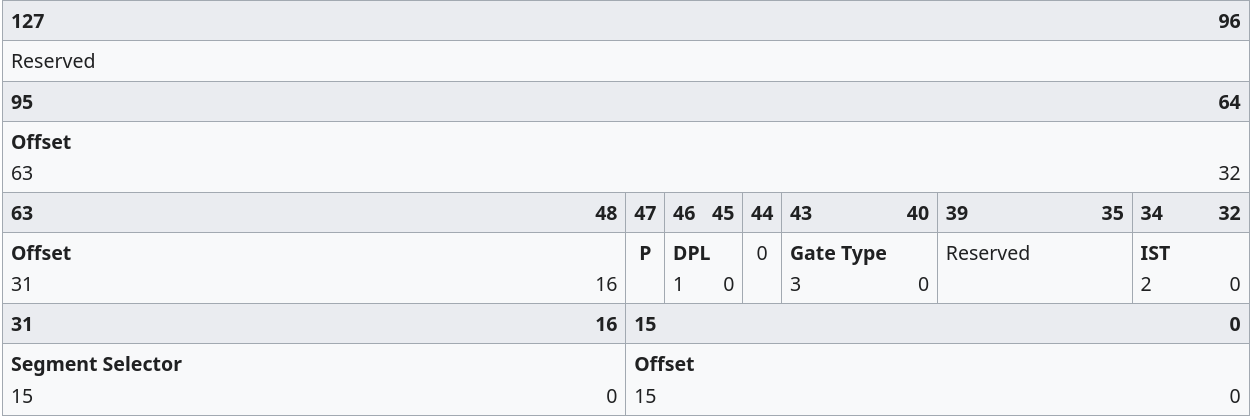
\includegraphics[scale=0.2]{../figures/entrata_idt.png}
\end{center}

\subsubsection{Gestione dell'interruzione software}
Avevamo visto come il meccanismo dell'interruzione, definito un gate nella IDT, si riduceva al caricamento in RIP dell'indirizzo del gestore e dell'immissione in pila dei seguenti dati:
\begin{table}[H]
	\center
	\begin{tabular} { c | p{5cm} }
		\lstinline|0| & RIP \\
		\lstinline|+1| & CS \\
		\lstinline|+2| & RFLAGS 
	\end{tabular}
\end{table}
Cioè si impostava un nuovo frame sulla pila con i seguenti dati:
\begin{itemize}
	\item L'instruction pointer \textbf{RIP}, da dove si vorrà ripartire nell'esecuzione una volta gestita l'interruzione.
		Notiamo che in verità questo indirizzo, che è fra l'altro in memoria virtuale, è corredato a seconda del tipo di gate dall'\textbf{SS} (\textit{Stack Segment}) o dal \textbf{TSS} (\textit{Task State Segment}), utili alla memoria segmentata che come abbiamo visto non ci è di interesse. La caratteristica importante è che si conserva un riferimento a dove ripartire, in memoria, nell'esecuzione una volta gestita l'interruzione;
	\item Il contenuto attuale di \textbf{CS}, cioè il contesto al momento della chiamata, che chiaramente vorremo ristabilire in seguito;
	\item Come abbiamo visto, anche \textbf{RFLAGS} viene memorizzato, in quanto gli interrupt mascherabili vengono mascherati in fase di gestione di un interrupt sistema (attraverso il flag \textbf{IF}), e vogliamo resettare questo comportamente al termine della gestione.
\end{itemize}

A questo punto l'unica differenza nella chiamata di interrupt in caso di cambio di contesto sta effettivamente nella transizione fra due \textbf{pile}: la separazione fra contesto utente e contesto sistema viene infatti resa possibile anche dalla presenza di due pile separate, di cui l'ultima chiaramente sta in memoria protetta.
Il programma è normalmente in esecuzione nella pila utente: al momento del sollevamento di un interruzione software, si passa all'esecuzione (se alcune condizioni che vedremo fra poco sono rispettate) della routine di gestione definita dal sistema operativo.
Questo richiede un modo per preservare la posizione della pila utente, da cui ci spostiamo quando passiamo alla pila sistema.
Facciamo ciò conservando il vecchio \textbf{RSP}, immettendolo in pila prima dei registri visti prima, cioè creando un frame del tipo:
\begin{table}[H]
	\center
	\begin{tabular} { c | p{7cm} }
		\lstinline|0| & RIP \\
		\lstinline|+1| & CS \\
		\lstinline|+2| & RFLAGS \\ 
		\lstinline|+3| & RSP (Pila utente)
	\end{tabular}
\end{table}
Il vecchio valore di RSP permetterà, fra l'altro, di accedere e modificare il contesto del \textit{processo} in esecuzione con la sua pila utente.

Un caso particolare ma permesso è rappresentato dalla situazione dove \textbf{L}, il livello di destinazione, corrisponde allo stato attuale (ad esempio, sono permesse chiamate di interruzioni da contesto utente a contesto utente, o da contesto sistema a contesto sistema).
In questo caso, chiaramente, tutta questa operazione verrà svolta su un unica pila (sia questa la pila utente o la pila sistema).
Noteremo fra poco come questa possibilità rivela delle falle di sicurezza che vanno gestite.

\subsubsection{Transizione da contesto sistema a contesto utente}
La transizione inversa a quella vista adesso viene fatta semplicemente ritornando dall'interruzione attraverso la \lstinline|IRETQ|.
In questo caso si preleva dalla pila sistema (utente se eravamo in un interruzione a gestione livello utente) le informazioni che vi avevamo inserito al momento della chiamata dell'interruzione (RIP, CS ed EFLAGS) e si ristabilisce lo stato precedente al sollevamento dell'istruzione.
Anche qui vi sono delle particolarità, che verranno spiegato, assieme a quelle annunciate in precedenza, nel paragrafo seguente.

\subsubsection{Particolarità della gestione delle interruzioni software}
Notiamo una particolarità riguardo alla transizione di contesto in fase di chiamata dell'interruzione (nota osservando il contesto attuale e l'L dell'interruzione lanciata), e riguardo alla transizione di contesto in fase di ritorno dall'interruzione (nota osservando il contesto attuale e il contesto salvato in pila).

Infatti, in fase di chiamata (quando si usa la \lstinline|INT|), se L è minore del contesto corrente, viene lanciato un errore.
La motivazione è principalmente una questione di simmetria nel meccanismo di chiamata delle interruzioni, piuttosto che una ragione di sicurezza: si vuole che le interruzioni ci portino in contesti maggiori o uguali del livello presente in CS.

Viceversa, se si prova a passare ad un livello superiore in fase di ritorno dall'interuzione (cioè quando si usa la \lstinline|IRETQ|), viene lanciato un altro errore.
La motivazione è che, visto che prevediamo nell'IDT il flag L, livello di destinazione, che permette di chiamare interruzioni in contesto utente, l'utente potrebbe impostare un frame di pila dove si richiede effettivamente l'accesso ad un livello di protezione superiore, e poi usare \lstinline|IRETQ| per ritornare da tale frame di pila e passare quindi a tale livello di accesso.

\end{document} 
